\usetikzlibrary{arrows}
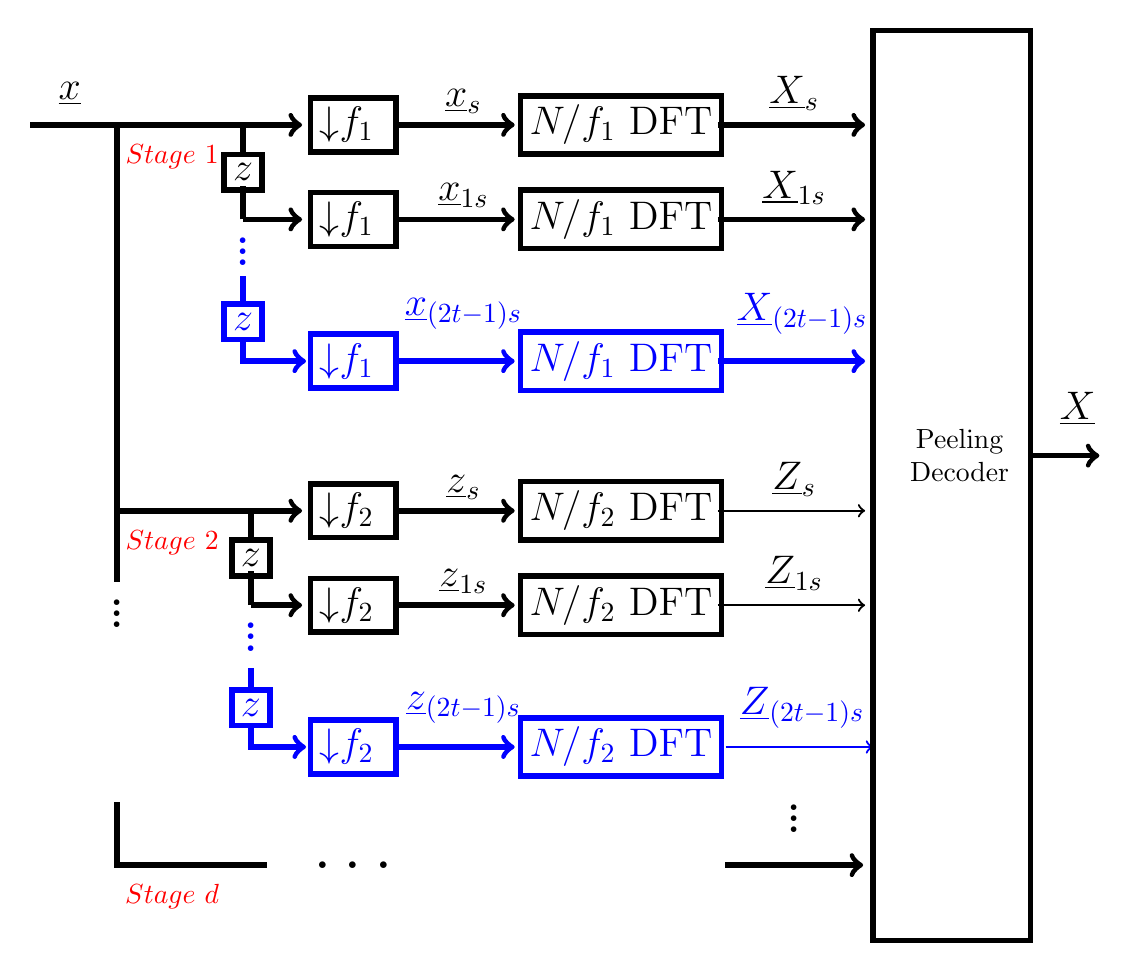
\begin{tikzpicture}

 % Downsampling blocks
\node[draw,align=center,thick,line  width =2pt] at (1,4.5) {\Large{$\mathbf{\downarrow} f_2$} };
\node[draw,align=center,thick,line  width =2pt] at (1,5.7) {\Large{$\mathbf{\downarrow} f_2$ }};
\node[draw,align=center,thick,blue,line  width =2pt] (v6) at (1,2.7) {\Large{$\mathbf{\downarrow} f_2$ }};

\node[draw,align=center,thick,line  width =2pt] at (1,9.4) {\Large{$\mathbf{\downarrow} f_1$} };
\node[draw,align=center,thick,line  width =2pt] at (1,10.6) {\Large{$\mathbf{\downarrow} f_1$ }};
\node[draw,align=center,thick,blue,line  width =2pt] at (1,7.6) {\Large{$\mathbf{\downarrow} f_1$ }};

%  Input lines to the down-sampling block
 \draw[->,thick,line  width =2pt] (-0.3,4.5) -- (0.35,4.5);
 \draw[->,thick,line  width =2pt] (-0.3,5.7) -- (0.35,5.7);
  
 \draw[->,thick,line  width =2pt] (-0.4,9.4) -- (0.35,9.4);
 \draw[->,thick,line  width =2pt] (-0.4,10.6) -- (0.35,10.6);

%  Delay blocks
\node[draw,align=center,thick,line  width =2pt] at (-0.3,5.1) {\Large{$z$}};
\node[draw,align=center,thick,line  width =2pt] at (-0.4,10) {\Large{$z$}};
\node[draw,align=center,thick,blue,line  width =2pt] (v7) at (-0.3,3.2) {\Large{$z$}};
\node[draw,align=center,thick,blue,line  width =2pt] at (-0.4,8.1) {\Large{$z$}};

% paths connecting the delay blocks
 \draw[thick,line  width =2pt] (-0.3,4.5) -- (-0.3,4.93);
 \draw[thick,line  width =2pt] (-0.3,5.3) -- (-0.3,5.7);


\node[blue,line  width =2pt] at (-0.4,9.1) {\Huge${\vdots}$};
\node[blue,line  width =2pt] at (-0.3,4.2) {\Huge${\vdots}$};
 
 \draw[thick,line  width =2pt] (-0.4,9.4) -- (-0.4,9.83);
 \draw[thick,line  width =2pt] (-0.4,10.2) -- (-0.4,10.6);
 
% paths connecting the two stages   
 \draw[thick,line  width =2pt] (-0.4,10.6) -- (-2,10.6);
 \draw[thick,line  width =2pt] (-0.3,5.7) -- (-2,5.7);
 \draw[thick,line  width =2pt] (-2,5.7) -- (-2,10.6);
  \draw[thick,line  width =2pt] (-3.1,10.6) -- (-2,10.6);
  \draw[thick,line  width =2pt] (-2,5.7) -- (-2,4.8);
  
  
  % DFT blocks
\node[draw,align=center,thick,line  width =2pt] at (4.4,4.5) {\Large{$N/f_2$ DFT}};
\node[draw,align=center,thick,line  width =2pt] at (4.4,5.7) {\Large{$N/f_2$ DFT}};
\node[draw,align=center,thick,blue,line  width =2pt] at (4.4,2.7) {\Large{$N/f_2$ DFT}};

\node[draw,align=center,thick,line  width =2pt] at (4.4,9.4) {\Large{$N/f_1$ DFT}};
\node[draw,align=center,thick,line  width =2pt] at (4.4,10.6) {\Large{$N/f_1$ DFT}};
\node[draw,align=center,thick,blue,line  width =2pt] at (4.4,7.6) {\Large{$N/f_1$ DFT}};
% Connectors
 \draw[->,thick,line  width =2pt] (1.55,10.6) -- (3.05,10.6);
 \draw[->,thick,line  width =2pt] (1.55,9.4) -- (3.05,9.4);
 \draw[->,thick,blue,line  width =2pt] (1.55,7.6) -- (3.05,7.6);
 
 \draw[->,thick,line  width =2pt] (1.55,5.7) -- (3.05,5.7);
 \draw[->,thick,line  width =2pt] (1.55,4.5) -- (3.05,4.5);
 \draw[->,thick,blue,line  width =2pt] (1.55,2.7) -- (3.05,2.7);

 \draw[->,thick,line  width =2pt] (5.63,10.6) -- (7.5,10.6);
 \draw[->,thick,line  width =2pt] (5.63,9.4) -- (7.5,9.4);
 \draw[->,thick,blue,line  width =2pt] (5.63,7.6) -- (7.5,7.6);
 
 \draw[->,thick] (5.63,5.7) -- (7.5,5.7);
 \draw[->,thick] (5.63,4.5) -- (7.5,4.5);
 \draw[->,thick,blue] (5.73,2.7) -- (7.6,2.7);
 
  % Labels
  \node[draw=none,align=center] at (-2.6,11) {\Large{$\underline{x}$}};
  
  \node[draw=none,align=center] at (2.4,10.9) {\Large{$\underline{x}_{s}$}};
  \node[draw=none,align=center] at (2.4,9.7) {\Large{$\underline{x}_{1s}$}};
\node[draw=none,align=center,blue] at (2.4,8.2) {\Large{$\underline{x}_{(2t-1)s}$}};

\node[draw=none,align=center] at (2.4,6) {\Large{$\underline{z}_{s}$}};
  \node[draw=none,align=center] at (2.4,4.8) {\Large{$\underline{z}_{1s}$}};
  \node[draw=none,align=center,blue] at (2.4,3.2) {\Large{$\underline{z}_{(2t-1)s}$}};

  \node[draw=none,align=center] at (6.6,11) {\Large{$\underline{X}_{s}$}};
  \node[draw=none,align=center] at (6.6,9.8) {\Large{$\underline{X}_{1s}$}};
  \node[draw=none,align=center,blue] at (6.7,8.2) {\Large{$\underline{X}_{(2t-1)s}$}};
  
  \node[draw=none,align=center] at (6.6,6.1) {\Large{$\underline{Z}_{s}$}};
  \node[draw=none,align=center] at (6.6,4.9) {\Large{$\underline{Z}_{1s}$}};
  \node[draw=none,align=center,blue] at (6.7,3.2) {\Large{$\underline{Z}_{(2t-1)s}$}};
  
  \node [draw=none] at (-2,4.5) {\Huge${\vdots}$} ;
  
   \node[draw=none,align=center] at (-1.3,10.2) {\color{red}$Stage ~1$};
  \node[draw=none,align=center] at (-1.3,5.3) {\color{red}$Stage ~2$};
   \node[draw=none,align=center] at (-1.3,0.8) {\color{red}$Stage ~d$};
\draw [thick,line  width =2pt](-2,2) -- (-2,1.2) -- (-0.1,1.2) ;
 \node[draw=none,align=center] at (1,1.2) {\Huge${\ldots}$};
 
\draw [thick,line  width =2pt] (7.6,0.2424) rectangle (9.6,11.8);
\node (v1) at (5.6,1.2) {};
\node (v2) at (7.6,1.2) {};

\node (v5) at (-0.4,8.8) {};
\node (v8) at (-0.4,8.2) {};
\node (v9) at (-0.4,8) {};
\node (v11) at (0.5,7.6) {};
\node (v10) at (-0.4,7.6) {};

\draw  [->,thick,line  width =2pt](v1) edge (v2);
\node at (6.6,1.9) {\Huge${\vdots}$};
\node [text width=3cm, align =center ] at (8.7,6.4) {Peeling \\ Decoder};
\node (v3) at (9.5,6.4) {};
\node (v4) at (10.6,6.4) {};
\draw [thick, ->,line  width =2pt] (v3) edge (v4);
\node at (10.2,7) {\Large{$\underline{X}$}};

\draw [thick,blue,line  width =2pt] (v5) edge (v8);

\draw [thick,blue,->,line  width =2pt] (-0.4,7.9) -- (-0.4,7.6) -- (0.4,7.6);
\draw [thick,blue,->,line  width =2pt] (-0.3,3) -- (-0.3,2.7) -- (0.4,2.7);
\draw [thick,blue,line  width =2pt] (-0.3,3.7) -- (-0.3,3.4);
\end{tikzpicture}